\documentclass[notes,11pt, aspectratio=169, xcolor=table]{beamer}

\usepackage{pgfpages}
% These slides also contain speaker notes. You can print just the slides,
% just the notes, or both, depending on the setting below. Comment out the want
% you want.
\setbeameroption{hide notes} % Only slide
%\setbeameroption{show only notes} % Only notes
%\setbeameroption{show notes on second screen=right} % Both

\usepackage{helvet}
\usepackage[default]{lato}
\usepackage{array}
\usepackage{minted}

\newtheorem{proposition}{Proposition}
\usetikzlibrary{fillbetween}  % make sure this is loaded!

\usepackage{tikz}
\usetikzlibrary{shapes.geometric}
\usepackage{pgfplots}
\usepackage{graphicx}
\usepackage{verbatim}
\setbeamertemplate{note page}{\pagecolor{yellow!5}\insertnote}
\usetikzlibrary{positioning}
\usetikzlibrary{snakes}
\usetikzlibrary{calc}
\usetikzlibrary{arrows}
\usetikzlibrary{decorations.markings}
\usetikzlibrary{shapes.misc}
\usetikzlibrary{matrix,shapes,arrows,fit,tikzmark}
\usepackage{amsmath}
\usepackage{mathpazo}
\usepackage{hyperref}
\usepackage{lipsum}
\usepackage{multimedia}
\usepackage{graphicx}
\usepackage{multirow}
\usepackage{graphicx}
\usepackage{dcolumn}
\usepackage{bbm}
\usepackage[style=authoryear,sorting=nyt,uniquename=false]{biblatex}

\addbibresource{references.bib} 

\newcolumntype{d}[0]{D{.}{.}{5}}

\def\@@mybluebox[#1][#2]#3{
    \sbox\mytempbox{#3}%
    \mytemplen\ht\mytempbox
    \advance\mytemplen #1\relax
    \ht\mytempbox\mytemplen
    \mytemplen\dp\mytempbox
    \advance\mytemplen #2\relax
    \dp\mytempbox\mytemplen
    \colorbox{myblue}{\hspace{1em}\usebox{\mytempbox}\hspace{1em}}}


\usepackage{changepage}
\usepackage{appendixnumberbeamer}
\newcommand{\beginbackup}{
   \newcounter{framenumbervorappendix}
   \setcounter{framenumbervorappendix}{\value{framenumber}}
   \setbeamertemplate{footline}
   {
     \leavevmode%
     \hline
     box{%
       \begin{beamercolorbox}[wd=\paperwidth,ht=2.25ex,dp=1ex,right]{footlinecolor}%
%         \insertframenumber  \hspace*{2ex} 
       \end{beamercolorbox}}%
     \vskip0pt%
   }
 }
\newcommand{\backupend}{
   \addtocounter{framenumbervorappendix}{-\value{framenumber}}
   \addtocounter{framenumber}{\value{framenumbervorappendix}} 
}


\usepackage{graphicx}
\usepackage[space]{grffile}
\usepackage{booktabs}

% These are my colors -- there are many like them, but these ones are mine.
\definecolor{blue}{RGB}{0,114,178}
\definecolor{red}{RGB}{213,94,0}
\definecolor{yellow}{RGB}{240,228,66}
\definecolor{green}{RGB}{0,158,115}

\hypersetup{
  colorlinks=false,
  linkbordercolor = {white},
  linkcolor = {blue}
}


%% I use a beige off white for my background
\definecolor{MyBackground}{RGB}{255,253,218}

%% Uncomment this if you want to change the background color to something else
%\setbeamercolor{background canvas}{bg=MyBackground}

%% Change the bg color to adjust your transition slide background color!
\newenvironment{transitionframe}{
  \setbeamercolor{background canvas}{bg=yellow}
  \begin{frame}}{
    \end{frame}
}

\setbeamercolor{frametitle}{fg=blue}
\setbeamercolor{title}{fg=blue}
\setbeamertemplate{footline}[frame number]
\setbeamertemplate{navigation symbols}{} 
\setbeamertemplate{itemize items}{-}
\setbeamercolor{itemize item}{fg=blue}
\setbeamercolor{itemize subitem}{fg=blue}
\setbeamercolor{enumerate item}{fg=blue}
\setbeamercolor{enumerate subitem}{fg=blue}
\setbeamercolor{button}{bg=MyBackground,fg=blue,}



% If you like road maps, rather than having clutter at the top, have a roadmap show up at the end of each section 
% (and after your introduction)
% Uncomment this is if you want the roadmap!
% \AtBeginSection[]
% {
%    \begin{frame}
%        \frametitle{Roadmap of Talk}
%        \tableofcontents[currentsection]
%    \end{frame}
% }
\setbeamercolor{section in toc}{fg=blue}
\setbeamercolor{subsection in toc}{fg=red}
\setbeamersize{text margin left=1em,text margin right=1em} 

\newenvironment{wideitemize}{\itemize\addtolength{\itemsep}{10pt}}{\enditemize}

\usepackage{environ}
\NewEnviron{videoframe}[1]{
  \begin{frame}
    \vspace{-8pt}
    \begin{columns}[onlytextwidth, T] % align columns
      \begin{column}{.58\textwidth}
        \begin{minipage}[t][\textheight][t]
          {\dimexpr\textwidth}
          \vspace{8pt}
          \hspace{4pt} {\Large \sc \textcolor{blue}{#1}}
          \vspace{8pt}
          
          \BODY
        \end{minipage}
      \end{column}%
      \hfill%
      \begin{column}{.42\textwidth}
        \colorbox{green!20}{\begin{minipage}[t][1.2\textheight][t]
            {\dimexpr\textwidth}
            Face goes here
          \end{minipage}}
      \end{column}%
    \end{columns}
  \end{frame}
}

\title[]{International Trade: Data Lab 3}
\subtitle[]{Your first numerical model}
\author[Góes]
{Carlos Góes\inst{1}}
\date{Fall 2025}
\institute[GWU]{\inst{1} George Washington University }



\begin{document}

%%% TIKZ STUFF
\tikzset{   
        every picture/.style={remember picture,baseline},
        every node/.style={anchor=base,align=center,outer sep=1.5pt},
        every path/.style={thick},
        }
\newcommand\marktopleft[1]{%
    \tikz[overlay,remember picture] 
        \node (marker-#1-a) at (-.3em,.3em) {};%
}
\newcommand\markbottomright[2]{%
    \tikz[overlay,remember picture] 
        \node (marker-#1-b) at (0em,0em) {};%
}
\tikzstyle{every picture}+=[remember picture] 
\tikzstyle{mybox} =[draw=black, very thick, rectangle, inner sep=10pt, inner ysep=20pt]
\tikzstyle{fancytitle} =[draw=black,fill=red, text=white]
%%%% END TIKZ STUFF



%----------------------------------------------------------------------%
%-------------------       TITLE PAGE       ---------------------------%
%----------------------------------------------------------------------%





%----------------------------------------------------------------------%






%----------------------------------------------------------------------%
%----------------------------------------------------------------------%

%----------------------------------------------------------------------%
\frame{\titlepage}
\addtocounter{framenumber}{-1}
%----------------------------------------------------------------------%



%----------------------------------------------------------------------%
%----------------------------------------------------------------------%

\section{Introduction}

\begin{frame}{Plan for today}

\begin{wideitemize}
    \item Write down functions that map our model to the computer
    \item Input values for parameters
    \item Understand the logic of solving the model
    \item Try to solve it Python
\end{wideitemize}
    
\end{frame}


\begin{frame}{Factor and Goods Prices}
    \begin{wideitemize}
        \item Define $p = P_C / P_T$ to be the relative goods prices and $\omega = w_i /r_i$ to be the relative factor prices. 

        \item This is the same as defining $P_T=1$ to be the numeraire of this economy (dividing all prices for $P_T$)

        \item The following conditions still hold under free trade:

        \begin{equation*}
            \frac{K_{i,C}}{L_{i,C}} = 
      \underbrace{\frac{\beta_C}{1-\beta_C}}_{a_C}\;
      \omega,\qquad \frac{K_{i,T}}{L_{i,T}} = 
      \underbrace{\frac{\beta_T}{1-\beta_T}}_{a_T}\;
      \omega, \qquad a_T>a_C
        \end{equation*}

    \end{wideitemize}
\end{frame}

\begin{frame}{Frame Title}
    \begin{wideitemize}
        \item Recall that:

    \begin{eqnarray*}
        \frac{P_C}{P_T} &=& \frac{MPL_{i,T}}{MPL_{i,C}} \iff 
        \frac{P_C}{P_T} = \frac{(1-\beta_T) \times \left( \frac{K_{i,T}}{L_{i,T}} \right)^{\beta_T}}{ (1-\beta_C) \times \left( \frac{K_{i,C}}{L_{i,C}} \right)^{\beta_C}}  \\
    \frac{P_C}{P_T} &=& \frac{(1-\beta_T) \times \left( \frac{\beta_T}{1-\beta_T} \times \frac{w_i}{r_i}  \right)^{\beta_T}}{ (1-\beta_C) \times \left( \frac{\beta_C}{1-\beta_C} \times \frac{w_i}{r_i} \right)^{\beta_C}} \iff \frac{P_C}{P_T} = \underbrace{\frac{(1-\beta_T)^{1-\beta_T}\beta_T^{\beta_T}}
                          {(1-\beta_C)^{1-\beta_C}\beta_C^{\beta_C}}}_{\Phi}
          \;\omega^{\,\beta_T-\beta_C}
\end{eqnarray*} 

    \item Which means we can write relative factor prices as a function of relative goods prices (you know that!):

    \begin{equation*}
    \boxed{
        \omega(p) \equiv \Bigl(\tfrac{p}{\Phi}\Bigr)^{1/(\beta_T-\beta_C)}
    }
    \end{equation*}

    \end{wideitemize}
\end{frame}

\begin{frame}{Labor allocation}

\begin{wideitemize}
    \item Using the resource constraint and replacing for the relationship between capital-to-labor ratio and relative factor prices:

\begin{equation*}
   \bar{K}_i = \frac{K_{i,C}}{L_{i,C}} \times L_{i,C} + \frac{K_{i,T}}{L_{i,T}} \times (\bar{L}_i-L_{i,C}) \iff  \bar{K}_i  = a_C\times \omega  \times L_{i,C} + a_T \times \omega \times (\bar{L}_i-L_{i,C})
\end{equation*}

\item solving for $L_{i,C}$, we can write labor shares as a function of $\omega$ and, therefore, relative prices $p$:

\begin{equation*}\label{eq: lc}
    \boxed{
    L_{i,C}(p) = \frac{\bar{K}_i - a_T \times \omega(p) \times \bar{L}_i}{(a_C- a_T) \times \omega(p)}, \qquad L_{i,T}(p) = \bar{L}_i - L_{i,C}(p)
    }
\end{equation*}

\end{wideitemize}
    
\end{frame}

\begin{frame}{Production}

\begin{wideitemize}
\item Now note that we can write the production function in sector $g$ as:

\begin{equation*}
    Y_{i,g} = K_{i,g}^{\beta_g} L_{i,g}^{1-\beta_g} = \left(\frac{K_{i,g}}{L_{i,g}}\right)^{\beta_g} L_{i,g} =  \left(a_g \times \omega\right)^{\beta_g} L_{i,g} 
\end{equation*}

\item So output in each country-sector is a function of relative prices:

\begin{equation*}
\boxed{
    Y_{i,g}(p) =  \left(a_g \times \omega(p) \right)^{\beta_g} L_{i,g}(p) 
}
\end{equation*}
\end{wideitemize}
    
\end{frame}

\begin{frame}{Relative Supply}
    \begin{wideitemize}
        
\item So we can then characterize the relative supply function as a function of relative prices:

\begin{equation*}
\boxed{
    RS(p) = \frac{Y_{H,C}\left(p\right) + Y_{F,C}\left(p\right)}{Y_{H,T}\left(p\right) + Y_{F,T}\left(p\right)}
}
\end{equation*}

    \end{wideitemize}
\end{frame}

\begin{frame}{Relative Demand}

\begin{wideitemize}
    
\item From demand functions:

\begin{equation*}
    Q_{i,C} = \alpha  \frac{I_i}{P_{C}}, \qquad Q_{i,T} = (1-\alpha) \frac{I_i}{P_{T}}
\end{equation*}

\item Therefore:

\begin{equation*}
    \frac{Q_{H,C} + Q_{F,C} }{Q_{H,T}  + Q_{F,T} } = \frac{\alpha I_H/P_C + \alpha I_F/P_C}{(1-\alpha) I_H/P_T + (1-\alpha) I_F/P_T} = \frac{\alpha}{1-\alpha} \frac{I_H + I_F}{I_H + I_F} \frac{1}{P_C/P_T}
\end{equation*}

So we can express relative demand as a function of prices:

\begin{equation*}
    \boxed{
    RD(p) = \frac{\alpha}{1-\alpha} \frac{1}{p}
    }
\end{equation*}

\end{wideitemize}
    
\end{frame}


\begin{frame}[fragile=singleslide]{From theory to computing}

\begin{wideitemize}
    \item First let us define the parameters:

        \begin{minted}{python}
        beta_C, beta_T = 1 / 3, 2 / 3
        alpha = 0.5
        K   = {'H':4.0, 'F':3.0}      # capital endowments
        L   = {'H':8.0, 'F':2.0}      # labor endowments
        \end{minted}    

    \item and the constants

        \begin{minted}{python}
        a_C = beta_C / (1 - beta_C)
        a_T = beta_T / (1 - beta_T)
        Phi = (
            ((1 - beta_T) ** (1 - beta_T) * beta_T ** beta_T)
            / ((1 - beta_C) ** (1 - beta_C) * beta_C ** beta_C)
        )
        \end{minted}    

\end{wideitemize}
    
\end{frame}


\begin{frame}[fragile=singleslide]{From goods to factor prices}

    \begin{equation*}
    \boxed{
        \omega(p) \equiv \Bigl(\tfrac{p}{\Phi}\Bigr)^{1/(\beta_T-\beta_C)}
    }
    \end{equation*}

        
        \begin{minted}{python}
            def omega(p):
                """Solve ω from p = \Phi \omega^{β_T-β_C}."""
                exponent = 1.0 / (beta_T - beta_C)
                return (p / Phi) ** exponent
        \end{minted}    

\end{frame}

\begin{frame}[fragile=singleslide]{Labor Market}
\begin{equation*}\label{eq: lc}
    \boxed{
    L_{C}(i,p) = \frac{\bar{K}_i - a_T \times \omega(p) \times \bar{L}_i}{(a_C- a_T) \times \omega(p)}, \qquad L_{T}(i,p) = \bar{L}_i - L_{i,C}(p)
    }
\end{equation*}

        \begin{minted}{python}
        def L_C(i, omega):
            """Labour allocated to cloth in one country."""
            return (K[i] - a_T * omega * L[i]) / ((a_C - a_T) * omega)
        
        def L_T(i, omega):
            """Labour allocated to tech in one country."""
            return L[i] - L_C(i, omega)
        \end{minted}
    
\end{frame}

\begin{frame}[fragile=singleslide]{Production}

\begin{itemize}
    \item Output in each country-sector is a function of relative prices:

        \begin{equation*}
        \boxed{
            Y_{g}(i,p) =  \left(a_g \times \omega(p) \right)^{\beta_g} L_{g}(i,p)
        }
        \end{equation*}

        \begin{minted}{python}
        def Y_T(i, omega):
            return (a_T * omega)**beta_T * L_T(i, omega)
        
        def Y_C(i, omega):
            return (a_C * omega)**beta_C * L_C(i, omega)        
        \end{minted}
\end{itemize}
    
\end{frame}


\begin{frame}[fragile=singleslide]{Relative Supply}

\begin{wideitemize}
    
    \item Relative supply:

    \begin{equation*}
    \boxed{
        RS(p) = \frac{Y_{C}(H,p) + Y_{C}(F,p)}{Y_{T}(H,p) + Y_{T}(F,p)}
    }
    \end{equation*}

    note that this sums over $\{ H, F \}$. Does not depend on $i$.
        \begin{minted}{python}
def RS(p):
    """Relative supply Y_C / Y_T as a function of price *p*."""
    num = sum(Y_C(i, omega(p)) for i in ['H','F'])
    den = sum(Y_T(i, omega(p)) for i in ['H','F'])
    return num / den
        \end{minted}
        
    
\end{wideitemize}

    
\end{frame}


\begin{frame}[fragile=singleslide]{Relative Demand}

\begin{wideitemize}
    
\begin{equation*}
    \boxed{
    RD(p) = \frac{\alpha}{1-\alpha} \frac{1}{p}
    }
\end{equation*}

    \begin{minted}{python}
def RD(p):
    return alpha / (1-alpha) * 1/p
    \end{minted}

        
    
\end{wideitemize}

    
\end{frame}

\begin{frame}{Trade Equilibrium: Global Demand and Supply}
\begin{figure}
    \centering
        \begin{tikzpicture}
        
    \pgfmathsetmacro{\beta}{1/3}
    \pgfmathsetmacro{\alpha}{0.5}

    \pgfmathsetmacro{\Zm}{1}
    \pgfmathsetmacro{\K}{4}
    
    \pgfmathsetmacro{\Za}{1}
    \pgfmathsetmacro{\T}{1}

    \pgfmathsetmacro{\Kf}{1}
    \pgfmathsetmacro{\Tf}{1}


    \pgfmathsetmacro{\Ps}{\Za/\Zm * ((1-\alpha)/\alpha * \T / \K)^(\beta)}   
    \pgfmathsetmacro{\Qs}{(1-\alpha)/\alpha / \Ps}

    \pgfmathsetmacro{\Psf}{\Za/\Zm * ((1-\alpha)/\alpha * \Tf / \Kf)^(\beta)}   
    \pgfmathsetmacro{\Qsf}{(1-\alpha)/\alpha / \Psf}

    \pgfmathsetmacro{\Psw}{\Za/\Zm * ((1-\alpha)/\alpha * ( ( \T + \Tf) / (\K+\Kf ) )^(\beta)}   
    \pgfmathsetmacro{\Qsw}{(1-\alpha)/\alpha / \Psw}

    \pgfmathsetmacro{\A}{(\Zm/\Za)^(1/\beta) * ((\K+\Kf)/(\T+\Tf))}
    
    

        \centering
        \begin{axis}[
            xlabel={Relative Quantity: \textcolor{red}{$\frac{Q_{H,C} + Q_{F,C}}{Q_{H,T} + Q_{F,T}}$}, \textcolor{blue}{$\frac{Y_{H,C} + Y_{F,C}}{Y_{H,T} + Y_{F,T}}$}},
            ymin=0, ymax=3,
            xmin=0, xmax=2,
            yticklabel=\empty,
            xticklabel=\empty,
            axis lines=left,
            enlargelimits=false,
            clip=false,
            axis on top,
            scaled x ticks=false,
            width=9cm, height=7cm,
            title style={font=\bfseries}
        ]
        

        % red demand curve
        \addplot[name path=red, domain=0.4:1.7, thick, red]
          {(1-\alpha)/\alpha / x};
        
        % blue supply curve, now written as y
        \addplot[name path=blue, domain=0.2:1.5, thick, blue]
          { (x/\A)^( \beta/(1-\beta) ) };
        
        % fill between them
        \addplot[blue!20] fill between[of=red and blue];
        
        \addplot[dashed, thick] coordinates {(0,\Psw) (\Qsw,\Psw)};
        \node[black, anchor=east] at (axis cs:0,\Psw) {\scriptsize $p^*$};
        \addplot[dashed, thick] coordinates {(\Qsw,\Psw) (\Qsw,0)};

        %\addplot[dashed] coordinates {(0,\Psw) (\Qsw,\Psw)};
        %\node[black] at (axis cs:-0.1,\Psw) {\small $(P_{M}^*/P_{A}^*)^{Trade}$};
        %\addplot[dashed] coordinates {(\Qsw,\Psw) (\Qsw,0)};
        % \node[black] at (axis cs:\Qs,-0.15) {\small $\textcolor{red}{RD_i} = \textcolor{blue}{RS_i}$};

        
        %\addplot[thick, dashed, domain=0:5] {0.5};
        
        \end{axis}
        
        \end{tikzpicture}
        \caption{World Trade Equilibrium}
    \label{fig: trade-eqm}
\end{figure}
\end{frame}

\begin{frame}{How to solve for prices?}

\begin{wideitemize}
    \item Define excess demand function:

    \begin{equation*}
        ED(p) = RS(p) - RD(p)
    \end{equation*}

    \item This should be strictly increasing in price (check the figure above) -- it only crosses zero once

    \item Equilibrium price $p^*$ defined as the price for which supply equals demand:

    \begin{equation*}
        ED(p^*) = 0 \iff RS(p^*) = RD(p^*)
    \end{equation*}
    
\end{wideitemize}


    
\end{frame}

\begin{frame}{Trade Equilibrium: Global Demand, Supply, and Excess Demand}
\begin{figure}
    \centering
        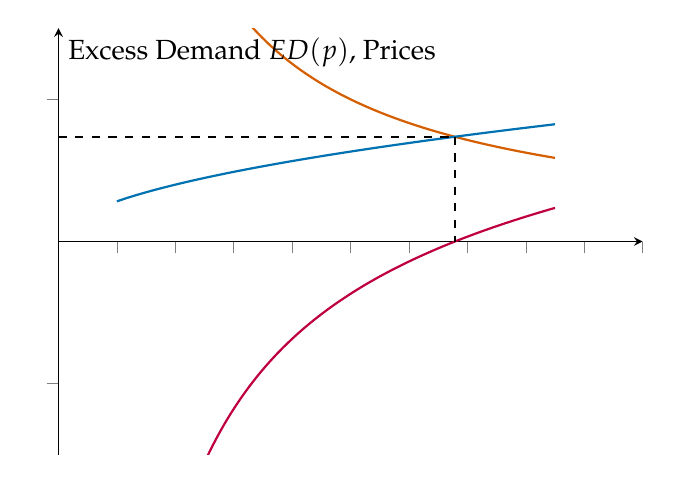
\begin{tikzpicture}
        
    \pgfmathsetmacro{\beta}{1/3}
    \pgfmathsetmacro{\alpha}{0.5}

    \pgfmathsetmacro{\Zm}{1}
    \pgfmathsetmacro{\K}{4}
    
    \pgfmathsetmacro{\Za}{1}
    \pgfmathsetmacro{\T}{1}

    \pgfmathsetmacro{\Kf}{1}
    \pgfmathsetmacro{\Tf}{1}


    \pgfmathsetmacro{\Ps}{\Za/\Zm * ((1-\alpha)/\alpha * \T / \K)^(\beta)}   
    \pgfmathsetmacro{\Qs}{(1-\alpha)/\alpha / \Ps}

    \pgfmathsetmacro{\Psf}{\Za/\Zm * ((1-\alpha)/\alpha * \Tf / \Kf)^(\beta)}   
    \pgfmathsetmacro{\Qsf}{(1-\alpha)/\alpha / \Psf}

    \pgfmathsetmacro{\Psw}{\Za/\Zm * ((1-\alpha)/\alpha * ( ( \T + \Tf) / (\K+\Kf ) )^(\beta)}   
    \pgfmathsetmacro{\Qsw}{(1-\alpha)/\alpha / \Psw}

    \pgfmathsetmacro{\A}{(\Zm/\Za)^(1/\beta) * ( (\K+\Kf) / (\T+\Tf) )}

    
    

        \centering
        \begin{axis}[
            axis lines=middle,
            yticklabel=\empty,
            xticklabel=\empty,
            ylabel={Excess Demand $ED(p)$, Prices},
            xmin=0, xmax=2,
            ymin=-1.5, ymax=1.5,
            samples=200,
            width=9cm, height=7cm,
            tick align=outside
        ]
        
        % demand
        \addplot[domain=.5:1.7, thick, purple]
        {(x/\A)^( \beta/(1-\beta) ) - ((1-\alpha)/\alpha) / x};

        \addplot[domain=0.4:1.7, thick, red]{(1-\alpha)/\alpha / x};
        % supply world
        \addplot[domain=0.2:1.7, thick, blue]{(x/\A)^(\beta/(1-\beta))};
        
        \addplot[dashed, thick] coordinates {(0,\Psw) (\Qsw,\Psw)};
        \node[black, anchor=east] at (axis cs:0,\Psw) {\scriptsize $p^*$};
        \addplot[dashed, thick] coordinates {(\Qsw,\Psw) (\Qsw,0)};

        %\addplot[dashed] coordinates {(0,\Psw) (\Qsw,\Psw)};
        %\node[black] at (axis cs:-0.1,\Psw) {\small $(P_{M}^*/P_{A}^*)^{Trade}$};
        %\addplot[dashed] coordinates {(\Qsw,\Psw) (\Qsw,0)};
        % \node[black] at (axis cs:\Qs,-0.15) {\small $\textcolor{red}{RD_i} = \textcolor{blue}{RS_i}$};

        
        %\addplot[thick, dashed, domain=0:5] {0.5};
        
        \end{axis}
        
        \end{tikzpicture}
\end{figure}
\end{frame}




\begin{frame}{Bisection Method}
\begin{figure}
    \centering
    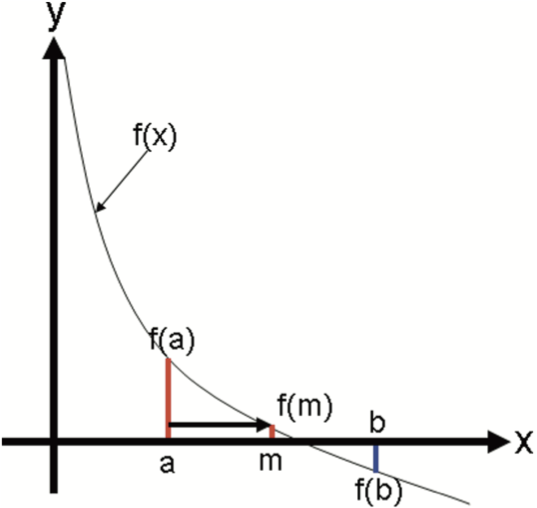
\includegraphics[width=0.5\linewidth]{figs/bisection-method.png}
    \caption{Root finding with bi-section method}
    \label{fig:ed}
\end{figure}
\end{frame}

\begin{frame}{Logic of algorithm}

\begin{wideitemize}
    \item Choose some small tolerance level $\varepsilon>0$ 
    
    \item Pick $a$, such that $ED(a) <0$ and $b$ such that $ED(b)>0$

    \item Calculate the median point $m = 1/2(a+b)$

    \item Calculate $ED(m)$

    \item If $ED(m)$ is positive ($ED(m)\times ED(a) <0$): update $b=m$

    \item If $ED(m)$ is negative ($ED(m)\times ED(a) \ge 0$): update $a=m$

    \item Repeat until $f(m) < \epsilon$

\end{wideitemize}
    
\end{frame}

\begin{frame}[fragile=singleslide]{Algorithm}

\begin{minted}{python}
    def bisect_root(f, a, b, tol=1e-6, max_iter=100):
    fa, fb = f(a), f(b)
    if fa*fb > 0:
        raise ValueError("Root not bracketed: f(a),f(b) same sign")
    for iter in range(max_iter):
        m = 0.5*(a+b)
        fm = f(m)
        if abs(fm) < tol or (b-a)<tol:
            return m
        if fa*fm < 0:
            b, fb = m, fm
        else:
            a, fa = m, fm
    raise RuntimeError("Bisection failed to converge")
\end{minted}

\end{frame}

\begin{frame}[fragile=singleslide]{Solve for prices}
    \begin{minted}{python}
p_low, p_high = 1, 1
# shrink/expand until signs differ
while excess_demand(p_low) > 0:
    p_low = p_low/2
while excess_demand(p_high) < 0:
    p_high = p_high*2

p_star = bisect_root(excess_demand, p_low, p_high)
omega_star = omega(p_star)
    \end{minted}
\end{frame}



\begin{frame}[fragile=singleslide]{Plot Excess Demand Function}
    \begin{minted}{python}
plt.style.use('fivethirtyeight')

# Declare figure
fig, ax = plt.subplots(figsize=(12,7))

x = np.linspace(0.5,1,100)
y = [excess_demand(i) for i in x]
# Plot line
plt.plot(x, y, color='red')
plt.axhline(0, color='black')
plt.axvline(p_star, color='black')
# Configure axes
ax.yaxis.grid(which="major", color='grey', linewidth=3)
ax.xaxis.grid(which="major", linewidth=0)
ax.tick_params(axis='both', which='major', labelsize=15)
plt.show()
    \end{minted}
\end{frame}

\begin{frame}{Excess Demand Function}
\begin{figure}
    \centering
    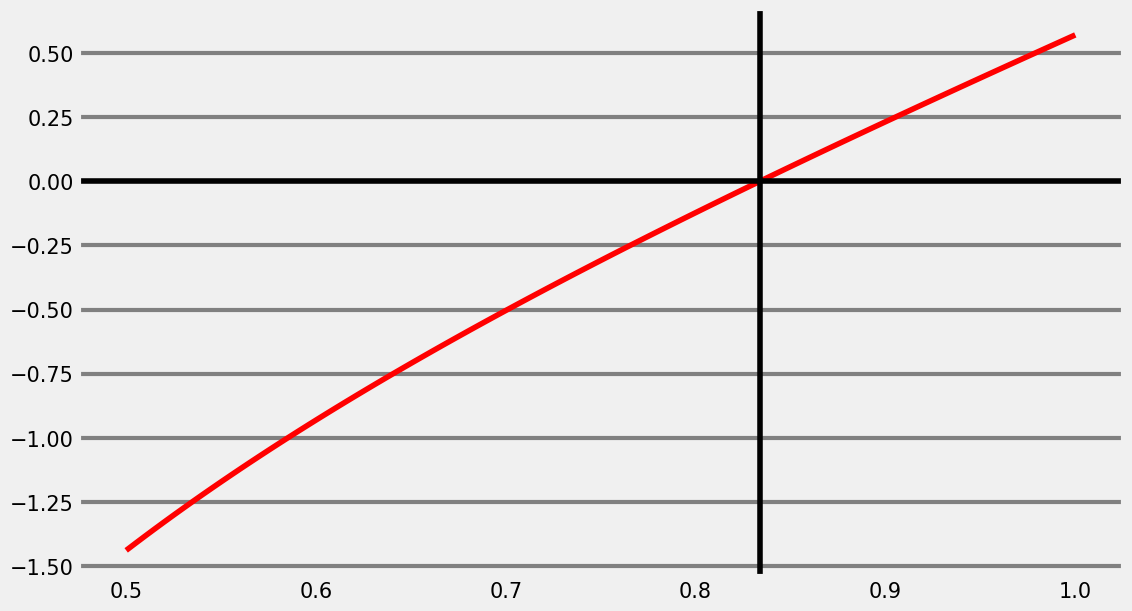
\includegraphics[width=0.75\linewidth]{figs/ed.png}
    \caption{Excess Demand Function}
    \label{fig:ed}
\end{figure}
\end{frame}


\end{document}



                xlabel={Relative Quantity: \textcolor{red}{$\frac{Q_{H,M} + Q_{F,M}}{Q_{H,A} + Q_{F,A}}$}, \textcolor{blue}{}},
